
%-----------------------------------------------------------------------------
% Chapter: System Design
%-----------------------------------------------------------------------------

\chapter{System Design}
\label{chap:SYSDES}

With all the key requirements being laid out in the previous chapter, it is
time to analyze them and draw a system design model on an abstract
level. 

\section{Specifications}
Non-functional requirements will be investigated first to decide the
non-behavioral specifications of the system, specifications like the
programming language and framework that powers the system, choice of database
management system (DBMS),
and the environment in which the system will be running.

\subsection{Frameworks}
Debate on whether or not it is better to use a framework never fails to be
a popular topic in the developer communities. On one hand, many developers
believe that a framework imposes a lot of constraints to a project which limits the
overall control of the project (especially core behaviors) \cite{frameworks}.
On the other hand, there are also many developers who believe that a framework
offers a better degree of efficiency and a better
measure of security to a project, while keeping the simplicity and
the architectural clarity of the project by enforcing the developers to apply
an architectural pattern (such as the \emph{model-view-controller} pattern
\cite{mvc}) to their code.

\medskip

Given the development time frame, requirements for
security and maintainability (see Sections~\ref{TIMEFRAME},
\ref{SECURITY}, and \ref{MAINTAINABILITY}),
as well as the scale of this project,
it is not unjustifiable for this project to use a web framework to achieve a
better result.

\medskip

The framework this project uses is called \emph{Django}, an open-source web
framework written in \emph{Python}. \emph{Django} was originally developed by
the web programming team at the \emph{Lawrence Journal-World} newspaper in 2003,
designed for the company to deliver their contents as fast as possible~\cite{django}.
With more than a decade of improvements
having been made to the framework, it is now among one of the most popular web
frameworks in the world, used by well-known companies and organizations like the
\emph{Washington Post}~\cite{djangoWashingtonPost}
and \emph{Instagram}~\cite{djangoInstagram}.
\medskip

The \emph{Django} framework provides a set of libraries to handle most basic
aspects of web application development. One good example of those libraries is
the \emph{object-relational mapper}. This framework has the capability to create
relational database schemas based on the \emph{Python} data model classes
written by the developer, so that no raw SQL query is required~\cite{django}
for most of the
database operations (such as select, filter, remove, and insert database
records).
This helps ensure that the possibility of having \emph{SQL Injection}
vulnerabilities is next to zero.

\subsection{DBMS}
The \emph{Course2018} LMS uses \emph{PostgreSQL} as the default database
management system, primarily because of its extensibility (such as direct
support of inheritance and document data types), which can be used for
development in the future of more advanced features without worrying about the
limitations of the DBMS~\cite{postgres}.

\medskip

Furthermore, if future developments really require a change of database
management system,
with the \emph{Django} framework's database libraries,
switching between different database management systems only requires
modification of a few lines of code in the project's settings file.

\subsection{Environment}
With the number of functional requirements (see Section~\ref{FUNCREQS}), it is not difficult for
one to foresee that there will be some external packages introduced to the
\emph{Course2018} LMS.
Additionally, it is highly possible that this system will be hosted
on a server along with other existing services; thus, to avoid packages that
are required for this system conflict with those existing services, an
isolated environment for this system is desired.

\medskip
The \emph{Django} project official guide~\cite{djangoGuide} recommends using
a tool called \texttt{virtualenv} to create an isolated environment. However,
this tool is only capable of isolating \emph{Python} packages, and the
\emph{Course2018} LMS may need to have some system packages (such as
compilers) isolated as well.

\medskip

Conventional virtualization (i.e., hardware virtualization) is a method for a
host computer system to simulate a hardware environment on which the guest
application can be run completely independent from the environment of the host
system, with dedicated resources from the host system~\citep[Chapter 16]{os}.
A \emph{virtual machine} (VM) could be a straightforward solution to solve
this,
but an efficient VM
(e.g., a \emph{kernel-based virtual machine}~\cite{kvm}) 
often places undesirable requirements to the host system 
(including a rebuild of the operating system kernel).

\subsubsection{Containerization}
\emph{Operating-system-level virtualization}, also known as
\emph{containerization}, is an operating system (OS) feature offered by the
kernel of the OS allowing multiple isolated user-space~\citep[Section 1.5.1]{os}
instances to exist simultaneously~\cite{docker};
each of these instances is known as a \emph{container}, and no dedicated resource
is required to be allocated for these instances.
This makes them much more
flexible than a conventional VM.
Further, with the same hardware system and
OS kernel as the host system being used, the overhead of a container is
generally considered to be next to nothing (compared to conventional VMs)~\cite{dockerVM}.

\pagebreak

Following are the results of the \texttt{uname} command
(a command to show the kernel version of a Unix or Unix-like OS)
on an \emph{Arch Linux} host system (Listing~\ref{lst:UNAME_HOST}),
a container on the host system with a \emph{Debian 8}~\cite{debian} image
(Listing~\ref{lst:UNAME_CONT}),
and a \emph{kernel-based VM} (KVM) on the host system with \emph{Debian 8} installed
(Listing~\ref{lst:UNAME_KVM}),
showing that containers share the same OS kernel with the host system whereas
VMs do not.


\begin{centering}
\lstinputlisting[caption=\texttt{uname} command on a \emph{Arch Linux} host system,
label=lst:UNAME_HOST, numbers=none]{./examples/uname-host.txt}
\lstinputlisting[caption=\texttt{uname} command in a containerized \emph{Debian}
environment,
label=lst:UNAME_CONT, numbers=none]{./examples/uname-container.txt}
\lstinputlisting[caption=\texttt{uname} command in a \emph{Debian} KVM,
label=lst:UNAME_KVM, numbers=none]{./examples/uname-kvm.txt}
\end{centering}

\subsubsection{Docker}
The \emph{Course2018} LMS is encapsulated in a container based on a
\emph{Debian} image, using a container management system called \emph{Docker}
which is an open-source implementation of \emph{OS-level~VM} developed by
\emph{Docker Inc}.

\medskip

With \emph{Docker}, the finished product of the
\emph{Course2018} LMS, along with all its dependencies, can be packed, shipped
and run on any host system with almost the same environment
(except for the OS kernel and the hardware environment)
as it was on the
developer's computer system. Therefore, the deployment process of the
\emph{Course2018} LMS will be as simple as typing just one command.

\need 1 in


\section{System modules}

As per requirements in Section~\ref{FUNCREQS}, the \emph{Course2018} LMS is composed of the
following modules.

\subsection{User authentication}
\label{sec:USRAUTH}
The \emph{Course2018} LMS uses the \emph{Django User Model} \cite{djangoUser}
to provide
basic functionalities related to user authentication activities, such as
user registration, user account management and user login/logout.
Each user account is attached with a profile containing the \emph{role}
(i.e., student or instructor) of the user. This \emph{role} attribute helps
the system perform permission control, such as to
decide whether or not a user has permission to access content
that does not belong to him; e.g., an instructor can view all students' assignment
files, but students can only view their own files.

\medskip

It is worth mentioning that there is no such role choice as a \emph{teaching
assistant}~(TA) defined in the profile model;
the reason behind this design decision is that all users can be defined as either a
student or an instructor without the knowledge of the courses in which they are
registered, but TAs are always associated with courses. That is, a user
can be a student or instructor in the \emph{Course2018} LMS, but he can only
be a TA for some specific courses.
Therefore, in the \emph{Course2018} LMS, the TA role is
reflected by a \emph{many-to-many} relationship between users and courses.

\subsection{File management}
The \emph{Django} official documentation recommends storing files in what is
called a ``\emph{Media directory}''. This directory will then be served by the
\emph{HTTP} server \cite{djangoManagingFiles}
(such as \emph{Apache} or \emph{Nginx}). However, this method does not allow
\emph{Django} to perform permission control on each individual file.

\medskip

To overcome this, the \emph{Course2018} LMS manages all users' files without
involving the \emph{HTTP} server by implementing a routine to provide file
download service to the users. Whenever a user requests access to a file, the system
will always perform a permission check before invoking that routine
(see Chapter \ref{chap:DEV} for more detail).

\medskip

In comparison with
using the \emph{HTTP} server (which is implemented in \emph{C}) to provide
the file download service,
implementing the same service in \emph{Python} is suboptimal in terms of
performance.
However, considering the fact that most of the course-related
files are relatively small, the performance difference should
not be significant.

\subsection{Files display}
Every time the \emph{Course2018} LMS receives a \emph{view file} request,
it invokes routines in the \emph{file management} module to locate the
requested file, then invokes this module to determine whether or not the
requested file can be displayed (e.g., a PDF file or a plain text file). Also,
if the requested file is a plaintext file, this module will try to determine
the programming language of the file and provide syntax highlighting for the
user.

\subsection{Course management}
This module is designed primarily for instructors to manage their courses, 
that is, to provide features such as create courses, modify course information,
register students/TAs, and upload course materials.

\subsection{Assignment management}
\label{sec:ASNMAN}
This module handles all the assignment-related activities, such activities are
divided into three categories: \emph{instructor activities}, 
\emph{marker activities}, and \emph{student activities}.

\medskip 

Note that users who have permission to view and grade the students' assignments
(i.e., instructors and TAs)
are defined in the \emph{Course2018} LMS as \emph{markers}, the reason behind
this design is that such activities (view and grade assignments) can be
performed by both the instructor and the TAs of a course, and the implementation
of the permission check for the \emph{marker}'s views involves checking both
of the roles, which is different than the permission check for views that are
designed solely for instructors or students.

\medskip

\subsubsection{Instructor activities}
\begin{itemize}
    \item Create, delete, modify assignments
    \item Assign grading tasks to TAs
    \item Release assignments grades
\end{itemize}

\subsubsection{Student activities}
\begin{itemize}
    \item View assignment requirements
    \item Submit assignments
    \item View submitted files (including version differences)
    \item View grade and marker's feedback
\end{itemize}

\subsubsection{Marker activities}
\begin{itemize}
    \item View and grade assignments
\end{itemize}

\subsection{Automated test}
After an instructor enables automated test and provides test-related
information (e.g., compile command, run options, and test cases) for a
programming assignment,
every submission will be built (if required) and executed in a separate
containerized environment; that is, a different
container than the one in which the \emph{Course2018} LMS is running.
This process is done by a \emph{shell script} which is generated by the LMS
using the test data provided by the instructor. This script compares the
output of a student's program with the sample output (provided by the instructor
as part of a test case); the result of those comparisons will be available for
all relevant parties (i.e., the student who submitted files, the TA and
the instructor) as soon as the process is finished.

\subsection{Marking interface}
This module mainly provides an easy-to-use interface for the
purpose of easing the process of assignment feedback for markers.
The interface splits the screen into two sections: a file display section on the
left-hand side, and a comments editing section on the right-hand side.

\section{Modules dependencies}
Many of the modules in the \emph{Course2018} LMS depends on each other,
thus, a dependency tree to determine the order of the development
process is shown in Figure~\ref{fig:DEP}.

\bigskip\ \\

\begin{figure}[ht]
    \centering
    \caption{Modules dependencies}
    \label{fig:DEP}

    \usetikzlibrary{er, positioning, arrows}
    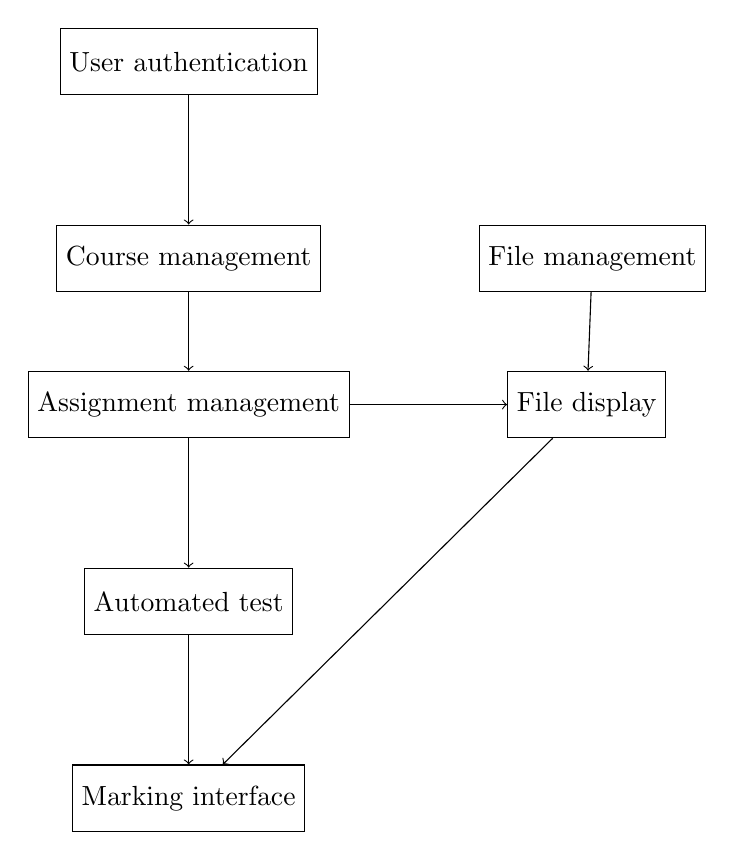
\begin{tikzpicture}[align=center, auto,node distance=2.5cm]
        \node[entity] (ua)      {User authentication};
    
        \node[entity] (cm) [below of = ua] {Course management};
        \node[entity] (am) [below = 1cm of cm] {Assignment management};
    
        \node[entity] (fm)  [right = 2cm of cm] {File management};
        \node[entity] (afd) [right = 2cm of am] {File display};
    
        \node[entity] (ct) [below of = am] {Automated test};
        \node[entity] (mk) [below of = ct] {Marking interface};
    
        \path[->] 
            (ua) edge node {} (cm)
            (fm) edge node {} (afd)
    
            (cm) edge node {} (am)
            (am) edge node {} (afd)
    
            (afd) edge node {} (mk)
            (am) edge node {} (ct)
    
            (ct) edge node {} (mk)
            ;
    \end{tikzpicture}
\end{figure}